% Created by tikzDevice version 0.12.3.1 on 2022-09-01 15:51:11
% !TEX encoding = UTF-8 Unicode
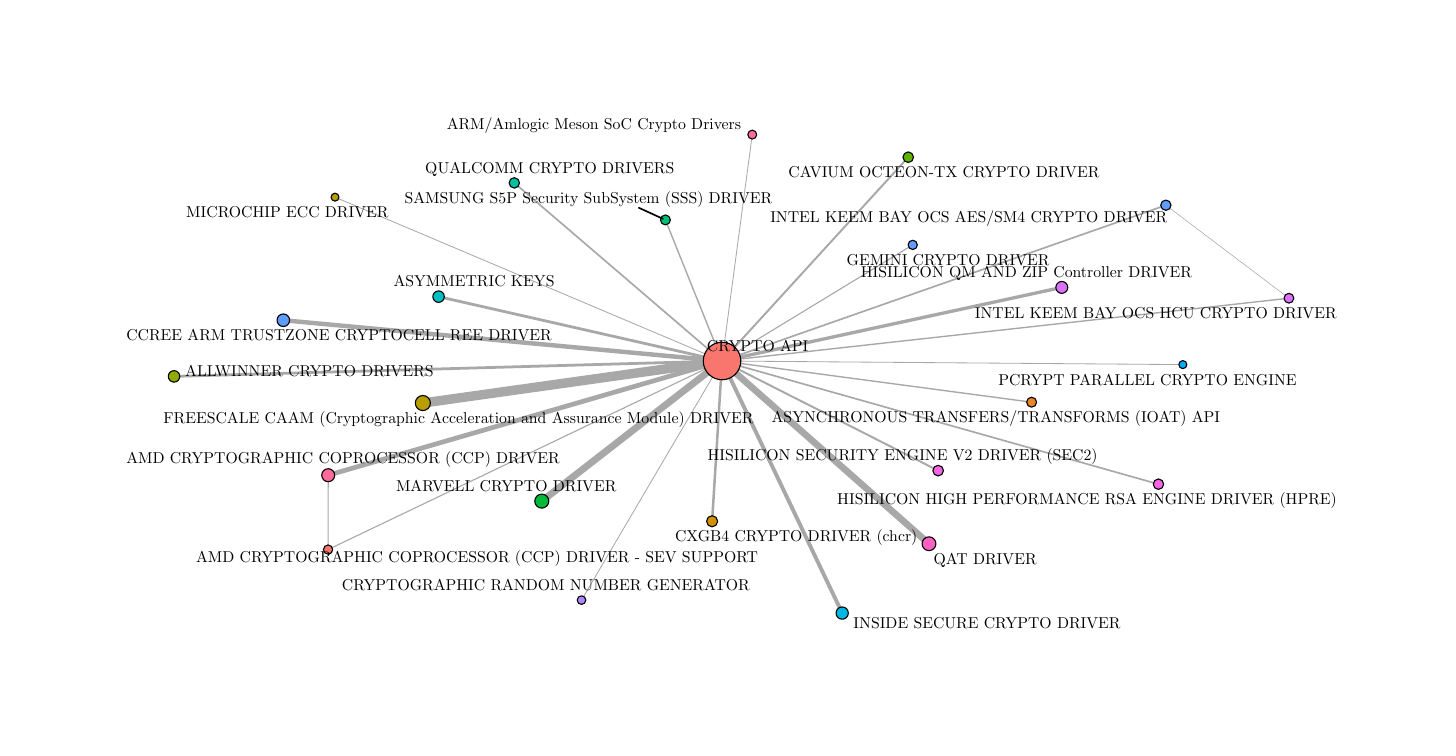
\begin{tikzpicture}[x=1pt,y=1pt]
\definecolor{fillColor}{RGB}{255,255,255}
\path[use as bounding box,fill=fillColor,fill opacity=0.00] (0,0) rectangle (505.89,252.94);
\begin{scope}
\path[clip] (  0.00,  0.00) rectangle (505.89,252.94);
\definecolor{fillColor}{RGB}{255,255,255}

\path[fill=fillColor] (  0.00,  0.00) rectangle (505.89,252.94);
\end{scope}
\begin{scope}
\path[clip] ( 32.75, 32.75) rectangle (475.89,222.94);
\definecolor{drawColor}{gray}{0.66}

\path[draw=drawColor,line width= 1.0pt,line join=round] ( 52.89,126.93) -- (250.91,132.49);

\path[draw=drawColor,line width= 0.4pt,line join=round] (108.60, 91.22) -- (108.55, 64.35);

\path[draw=drawColor,line width= 1.7pt,line join=round] (108.60, 91.22) -- (250.91,132.49);

\path[draw=drawColor,line width= 0.4pt,line join=round] (108.55, 64.35) -- (250.91,132.49);

\path[draw=drawColor,line width= 0.3pt,line join=round] (261.83,214.30) -- (250.91,132.49);

\path[draw=drawColor,line width= 1.0pt,line join=round] (148.48,155.75) -- (250.91,132.49);

\path[draw=drawColor,line width= 0.5pt,line join=round] (362.77,117.61) -- (250.91,132.49);

\path[draw=drawColor,line width= 0.7pt,line join=round] (318.19,206.13) -- (250.91,132.49);

\path[draw=drawColor,line width= 1.6pt,line join=round] ( 92.38,147.22) -- (250.91,132.49);

\path[draw=drawColor,line width= 0.3pt,line join=round] (250.91,132.49) -- (200.13, 46.09);

\path[draw=drawColor,line width= 0.9pt,line join=round] (250.91,132.49) -- (247.32, 74.58);

\path[draw=drawColor,line width= 3.4pt,line join=round] (250.91,132.49) -- (142.80,117.30);

\path[draw=drawColor,line width= 0.4pt,line join=round] (250.91,132.49) -- (319.81,174.45);

\path[draw=drawColor,line width= 0.6pt,line join=round] (250.91,132.49) -- (408.61, 87.98);

\path[draw=drawColor,line width= 1.2pt,line join=round] (250.91,132.49) -- (373.68,159.08);

\path[draw=drawColor,line width= 0.7pt,line join=round] (250.91,132.49) -- (329.00, 92.88);

\path[draw=drawColor,line width= 1.4pt,line join=round] (250.91,132.49) -- (294.32, 41.40);

\path[draw=drawColor,line width= 0.6pt,line join=round] (250.91,132.49) -- (411.28,188.79);

\path[draw=drawColor,line width= 0.5pt,line join=round] (250.91,132.49) -- (455.75,155.17);

\path[draw=drawColor,line width= 2.5pt,line join=round] (250.91,132.49) -- (185.77, 81.86);

\path[draw=drawColor,line width= 0.3pt,line join=round] (250.91,132.49) -- (111.06,191.69);

\path[draw=drawColor,line width= 0.3pt,line join=round] (250.91,132.49) -- (417.42,131.19);

\path[draw=drawColor,line width= 2.4pt,line join=round] (250.91,132.49) -- (325.69, 66.46);

\path[draw=drawColor,line width= 0.6pt,line join=round] (250.91,132.49) -- (175.84,196.85);

\path[draw=drawColor,line width= 0.5pt,line join=round] (250.91,132.49) -- (230.44,183.47);

\path[draw=drawColor,line width= 0.2pt,line join=round] (411.28,188.79) -- (455.75,155.17);
\definecolor{drawColor}{RGB}{0,0,0}
\definecolor{fillColor}{RGB}{147,170,0}

\path[draw=drawColor,line width= 0.4pt,line join=round,line cap=round,fill=fillColor] ( 52.89,126.93) circle (  2.07);
\definecolor{fillColor}{RGB}{255,105,156}

\path[draw=drawColor,line width= 0.4pt,line join=round,line cap=round,fill=fillColor] (108.60, 91.22) circle (  2.34);
\definecolor{fillColor}{RGB}{248,118,109}

\path[draw=drawColor,line width= 0.4pt,line join=round,line cap=round,fill=fillColor] (108.55, 64.35) circle (  1.67);
\definecolor{fillColor}{RGB}{255,105,156}

\path[draw=drawColor,line width= 0.4pt,line join=round,line cap=round,fill=fillColor] (261.83,214.30) circle (  1.61);
\definecolor{fillColor}{RGB}{0,191,196}

\path[draw=drawColor,line width= 0.4pt,line join=round,line cap=round,fill=fillColor] (148.48,155.75) circle (  2.07);
\definecolor{fillColor}{RGB}{232,133,38}

\path[draw=drawColor,line width= 0.4pt,line join=round,line cap=round,fill=fillColor] (362.77,117.61) circle (  1.80);
\definecolor{fillColor}{RGB}{94,179,0}

\path[draw=drawColor,line width= 0.4pt,line join=round,line cap=round,fill=fillColor] (318.19,206.13) circle (  1.91);
\definecolor{fillColor}{RGB}{97,156,255}

\path[draw=drawColor,line width= 0.4pt,line join=round,line cap=round,fill=fillColor] ( 92.38,147.22) circle (  2.27);
\definecolor{fillColor}{RGB}{248,118,109}

\path[draw=drawColor,line width= 0.4pt,line join=round,line cap=round,fill=fillColor] (250.91,132.49) circle (  6.78);
\definecolor{fillColor}{RGB}{174,135,255}

\path[draw=drawColor,line width= 0.4pt,line join=round,line cap=round,fill=fillColor] (200.13, 46.09) circle (  1.56);
\definecolor{fillColor}{RGB}{211,146,0}

\path[draw=drawColor,line width= 0.4pt,line join=round,line cap=round,fill=fillColor] (247.32, 74.58) circle (  2.01);
\definecolor{fillColor}{RGB}{183,159,0}

\path[draw=drawColor,line width= 0.4pt,line join=round,line cap=round,fill=fillColor] (142.80,117.30) circle (  2.72);
\definecolor{fillColor}{RGB}{97,156,255}

\path[draw=drawColor,line width= 0.4pt,line join=round,line cap=round,fill=fillColor] (319.81,174.45) circle (  1.67);
\definecolor{fillColor}{RGB}{245,100,227}

\path[draw=drawColor,line width= 0.4pt,line join=round,line cap=round,fill=fillColor] (408.61, 87.98) circle (  1.88);
\definecolor{fillColor}{RGB}{219,114,251}

\path[draw=drawColor,line width= 0.4pt,line join=round,line cap=round,fill=fillColor] (373.68,159.08) circle (  2.15);
\definecolor{fillColor}{RGB}{245,100,227}

\path[draw=drawColor,line width= 0.4pt,line join=round,line cap=round,fill=fillColor] (329.00, 92.88) circle (  1.92);
\definecolor{fillColor}{RGB}{0,185,227}

\path[draw=drawColor,line width= 0.4pt,line join=round,line cap=round,fill=fillColor] (294.32, 41.40) circle (  2.21);
\definecolor{fillColor}{RGB}{97,156,255}

\path[draw=drawColor,line width= 0.4pt,line join=round,line cap=round,fill=fillColor] (411.28,188.79) circle (  1.86);
\definecolor{fillColor}{RGB}{219,114,251}

\path[draw=drawColor,line width= 0.4pt,line join=round,line cap=round,fill=fillColor] (455.75,155.17) circle (  1.77);
\definecolor{fillColor}{RGB}{0,186,56}

\path[draw=drawColor,line width= 0.4pt,line join=round,line cap=round,fill=fillColor] (185.77, 81.86) circle (  2.53);
\definecolor{fillColor}{RGB}{183,159,0}

\path[draw=drawColor,line width= 0.4pt,line join=round,line cap=round,fill=fillColor] (111.06,191.69) circle (  1.43);
\definecolor{fillColor}{RGB}{0,173,250}

\path[draw=drawColor,line width= 0.4pt,line join=round,line cap=round,fill=fillColor] (417.42,131.19) circle (  1.45);
\definecolor{fillColor}{RGB}{255,97,195}

\path[draw=drawColor,line width= 0.4pt,line join=round,line cap=round,fill=fillColor] (325.69, 66.46) circle (  2.49);
\definecolor{fillColor}{RGB}{0,193,159}

\path[draw=drawColor,line width= 0.4pt,line join=round,line cap=round,fill=fillColor] (175.84,196.85) circle (  1.88);
\definecolor{fillColor}{RGB}{0,191,116}

\path[draw=drawColor,line width= 0.4pt,line join=round,line cap=round,fill=fillColor] (230.44,183.47) circle (  1.79);

\path[draw=drawColor,line width= 0.6pt,line join=round,line cap=round] (220.84,187.86) -- (229.57,183.86);

\node[text=drawColor,anchor=base,inner sep=0pt, outer sep=0pt, scale=  0.57] at (101.81,126.89) {ALLWINNER CRYPTO DRIVERS};

\node[text=drawColor,anchor=base,inner sep=0pt, outer sep=0pt, scale=  0.57] at (113.94, 95.37) {AMD CRYPTOGRAPHIC COPROCESSOR (CCP) DRIVER};

\node[text=drawColor,anchor=base,inner sep=0pt, outer sep=0pt, scale=  0.57] at (162.38, 59.67) {AMD CRYPTOGRAPHIC COPROCESSOR (CCP) DRIVER - SEV SUPPORT};

\node[text=drawColor,anchor=base,inner sep=0pt, outer sep=0pt, scale=  0.57] at (204.63,216.01) {ARM/Amlogic Meson SoC Crypto Drivers};

\node[text=drawColor,anchor=base,inner sep=0pt, outer sep=0pt, scale=  0.57] at (161.29,159.29) {ASYMMETRIC KEYS};

\node[text=drawColor,anchor=base,inner sep=0pt, outer sep=0pt, scale=  0.57] at (349.87,110.13) {ASYNCHRONOUS TRANSFERS/TRANSFORMS (IOAT) API};

\node[text=drawColor,anchor=base,inner sep=0pt, outer sep=0pt, scale=  0.57] at (331.09,198.64) {CAVIUM OCTEON-TX CRYPTO DRIVER};

\node[text=drawColor,anchor=base,inner sep=0pt, outer sep=0pt, scale=  0.57] at (112.52,139.73) {CCREE ARM TRUSTZONE CRYPTOCELL REE DRIVER};

\node[text=drawColor,anchor=base,inner sep=0pt, outer sep=0pt, scale=  0.57] at (263.77,136.05) {CRYPTO API};

\node[text=drawColor,anchor=base,inner sep=0pt, outer sep=0pt, scale=  0.57] at (187.25, 49.68) {CRYPTOGRAPHIC RANDOM NUMBER GENERATOR};

\node[text=drawColor,anchor=base,inner sep=0pt, outer sep=0pt, scale=  0.57] at (277.71, 67.11) {CXGB4 CRYPTO DRIVER (chcr)};

\node[text=drawColor,anchor=base,inner sep=0pt, outer sep=0pt, scale=  0.57] at (155.67,109.81) {FREESCALE CAAM (Cryptographic Acceleration and Assurance Module) DRIVER};

\node[text=drawColor,anchor=base,inner sep=0pt, outer sep=0pt, scale=  0.57] at (332.58,167.01) {GEMINI CRYPTO DRIVER};

\node[text=drawColor,anchor=base,inner sep=0pt, outer sep=0pt, scale=  0.57] at (382.79, 80.52) {HISILICON HIGH PERFORMANCE RSA ENGINE DRIVER (HPRE)};

\node[text=drawColor,anchor=base,inner sep=0pt, outer sep=0pt, scale=  0.57] at (360.88,162.62) {HISILICON QM AND ZIP Controller DRIVER};

\node[text=drawColor,anchor=base,inner sep=0pt, outer sep=0pt, scale=  0.57] at (316.14, 96.46) {HISILICON SECURITY ENGINE V2 DRIVER (SEC2)};

\node[text=drawColor,anchor=base,inner sep=0pt, outer sep=0pt, scale=  0.57] at (346.66, 35.76) {INSIDE SECURE CRYPTO DRIVER};

\node[text=drawColor,anchor=base,inner sep=0pt, outer sep=0pt, scale=  0.57] at (340.07,182.53) {INTEL KEEM BAY OCS AES/SM4 CRYPTO DRIVER};

\node[text=drawColor,anchor=base,inner sep=0pt, outer sep=0pt, scale=  0.57] at (407.64,147.71) {INTEL KEEM BAY OCS HCU CRYPTO DRIVER};

\node[text=drawColor,anchor=base,inner sep=0pt, outer sep=0pt, scale=  0.57] at (172.92, 85.41) {MARVELL CRYPTO DRIVER};

\node[text=drawColor,anchor=base,inner sep=0pt, outer sep=0pt, scale=  0.57] at ( 93.83,184.18) {MICROCHIP ECC DRIVER};

\node[text=drawColor,anchor=base,inner sep=0pt, outer sep=0pt, scale=  0.57] at (404.63,123.73) {PCRYPT PARALLEL CRYPTO ENGINE};

\node[text=drawColor,anchor=base,inner sep=0pt, outer sep=0pt, scale=  0.57] at (345.98, 58.97) {QAT DRIVER};

\node[text=drawColor,anchor=base,inner sep=0pt, outer sep=0pt, scale=  0.57] at (188.67,200.38) {QUALCOMM CRYPTO DRIVERS};

\node[text=drawColor,anchor=base,inner sep=0pt, outer sep=0pt, scale=  0.57] at (202.62,189.36) {SAMSUNG S5P Security SubSystem (SSS) DRIVER};
\end{scope}
\end{tikzpicture}
